\subsection{Logarithmic Transformation}

\[s=c\ \log(1+r)\]
\paragraph{}\label{note:note_about_log_base}
With attention to the explanation of `FIGURE 3.5' of Gonzalez, which
says logarithmic transformation with $c=1$ maps $[0,1.5 \times 10^6]$ to
$[0,6.2]$, we can say that \emph{base} of $\log$ in logarithmic transformation
is $10$. Although with attention to this formula, we can say `for each $b$ as
base of logarithm, we can find a proper $c$ to get the same results':
\[\log_b^x=\frac{\log_a^x}{\log_a^b}\]
Also note that \emph{Octave} uses Euler's Constant ($e$) as base for usual
\texttt{log} command. But for example, for diagrams which only contain simple
logarithms,  above equation says those are scaled with a constant.
\paragraph{}Gonzalez in his book says:
\begin{displayquote}
    this transformation maps a narrow range of low intensity values in the
    input into a wider range of output levels. 
\end{displayquote}
\paragraph{}Above means: `a narrow range into the wider range'. But does not say about:
\begin{itemize}
    \item which narrow range to which wider range?
    \item output of narrow range is lighter or darker than input?
\end{itemize}
\paragraph{Purpose}\label{purpose_of_logarithmic_transformation} of 
logarithmic transformation is increasing intensity of
dark pixels (a bit) and also decreasing intensity of light pixels (a bit). So
pixels that have low intensity will be more visible. 

\paragraph{}At first a question rises: Suppose we have an image \emph{A} with
intensities in $[0,255]$. We know $\log(1+A) \leq  \log(256) < 2.5$. So
intensities of output will be in an interval less than [0,3]. Now, why we say `a
narrow range into the wider range'? Also we know that $log(1+x) < x$. So why do
we say the logarithmic transformation will appear more details in darker pixels?

\paragraph{}The question may be investigated from two prospects:
\begin{enumerate}
    \item I think it is like comparing range of data type before and after a
    data type conversion. We know that logarithm function 
    is a monotonically increasing function, so if you get \emph{R} as range of
    original data type, then calculating 
    \begin{equation*}
        \frac{f(r) - f(min(R))}{f(max(R))-f(min(R))} - \frac{r -
        min(R)}{max(R)-min(R)}  \tag{*}
    \end{equation*}\label{relation:eq_1} 
    will be rational (note that because $f$ is monotonically increasing, so $f(max(R))-f(min(R))$ determines range of $f$ and 
    $max(R)-min(R)$ determines range of original data types):
    \begin{Verbatim}[frame=single,label=Octave lab:\ logarithmic-data-type-conversion]
        X=linspace (1,256,1000);
        Y=(log(X)/log(256))-(X-1)/256;
        plot(X,Y);   
    \end{Verbatim}
    For above sample code, see the \hyperref[note:note_about_log_base]{notes
    about base of logarithm bases}.
    \begin{figure}[htb!]
        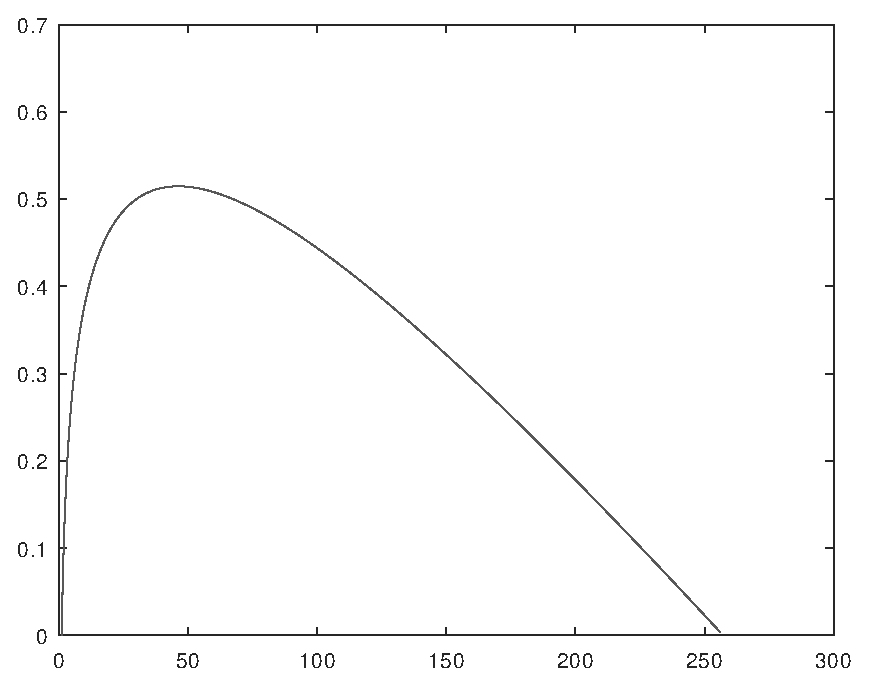
\includegraphics[scale=0.4]{logarithmic_transformation_data_type_conversion.eps}
        \centering
        \caption{logarithmic transformation data type conversion}
        \label{fig:logarithmic_transformation_data_type_conversion}
    \end{figure}
    
    As you can see in above figure, intensity of pixels in $[0,45]$ of $[0,
    255]$ will be mapped and streched to $[0,0.5]$ of $[0,1]$. The ratio of
    length of input to the total domain is $\frac{46}{256}$ and for output is 
    $\frac{0.5}{1}$. As you can see aspect ratio is increased (more than twice).
    Really the \hyperref[relation:eq_1]{*} formula, compars length of the
    interval $[0,r]$ and $[f(0), f(r)]$. Also 
    \autoref{fig:logarithmic_transformation_data_type_conversion} determines for
    logarithmic transformation, the length of output interval is always equal to
    or greater than input. It also determines difference between output and
    input intervals monotonically increases from $0$ up to $r=45$ and then
    decreases down to $0$.  
So we understand that the ratio of size of output of interval to the size of
range of logarithmic transformation is greater than or equal to the ratio of 
size of input to the size of input domain. So we can say the output is wider in 
its domain, or logarithmic transformation is an 
\gls{spatial_domain_glossary_label:intensity widening} transformation. 
And also we see that the intensity of output will be greater in its
color space (which is $[0,1]$) than intensity of input in its color space (which
is $[0,255]$), although the value of intensity of input is greater than
intensity of output. As ratio of intensity to length of color space determines
the pixel color in grayscale images, we understand why we say logarithmic
transformation will increase intensity of darker pixels. 
Also output of below sample code, which is shown in 
\autoref{fig:logarithmic_transformation_widening_and_compressing}, shows 
some of above facts. For example: the logarithmic transformation expands 
the $[0,50]$ of $[0,255]$ to the more than $60\%$ of target possible 
range\footnote{$(L-1) \times [0, 0.6]$} and $[150,255]$ to less than 
$20\%$ of upper limit of target range\footnote{$(L-1) \times [0.8, 1]$}:
\begin{Verbatim}[frame=single,label=Octave lab:\ Logarithmic transformation ]
    pkg load image;
    X=linspace (1,256,1000);
    Y=log(1+X);
    GY=mat2gray (Y);
    figure;plot(X,GY)
\end{Verbatim}
\begin{figure}[htb!]
    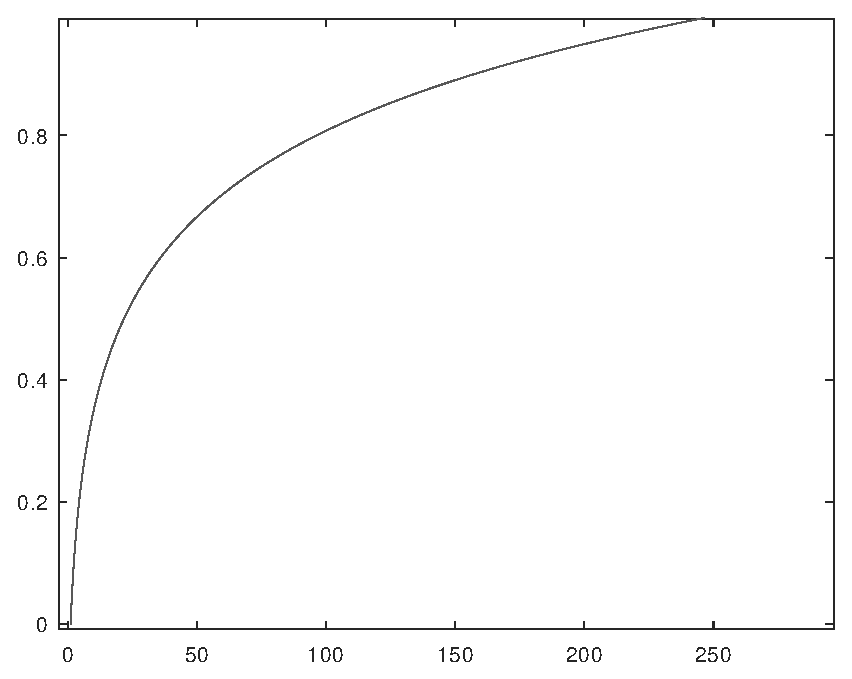
\includegraphics[scale=0.4]{logarithmic_transformation_widening_and_compressing.eps}
    \centering
    \caption{logarithmic transformation widening and compressing}
    \label{fig:logarithmic_transformation_widening_and_compressing}
\end{figure}
\item Now another question rises: Why \texttt{imhist(log(1+A))} only has a one
vertical line at $x=1$ and \texttt{imshow(log(1+A))} is white? This question
leads us to the second prospect which is related to 
\hyperref[Octave_notes_for_Logarithmic_transformation]
{Octave notes for Logarithmic transformation}.
 
\end{enumerate}

\subsubsection{Notes about details and quality}

As we saw before, logarithmic transformation is an 
\gls{spatial_domain_glossary_label:intensity widening}, 
so this satisfies the 
\hyperref[purpose_of_logarithmic_transformation]
{purpose of logarithmic transformation}. But what about lighter pixels? 
As \autoref{fig:logarithmic_transformation_widening_and_compressing} shows, 
logarithmic transformation compresses intensity of pixels which are in the range 
$[150,255]$. So:

\paragraph*{}\care
    If most of details are represented in pixels with higher intensity, then
    applying logarithmic transformation will cause in loss of 
    information\footnote{this is caused by both of human eye detection limits 
    and mathematical operation limits of computer which causes rounding.}. 


\subsubsection{Octave notes for Logarithmic transformation}
\label{Octave_notes_for_Logarithmic_transformation}

\paragraph{}The other prospect is relative to the way that a matrix be interpreted as an
image in \emph{Octave}: If the data type of matrix be double, then its range
must in $[0,1]$ and any data greater than 1 will be replaced by $1$ 
and any data less than $0$ will replaced by $0$. And if daata type is int,
range must be in $[0,255]$.

Now pay attention that data type of \texttt{log(1+A)} is double. So if you
interpret it as an image, all its data must be in $[0,1]$ and all data out
of that range will be replaced with $0$ or $1$. So we have to map
\texttt{log(1+A)} to $[0,1]$ while keeping the aspects ratio of data.
\texttt{im2double} does not work, because it only changes data when input be
of type int. The command \texttt{im2double(uint8(log(1+A)))} will be an
image in range $[0,1]$; but \emph{uint8} causes data loss and image will be
pixelized. So we have to use \texttt{mat2gray} command: 
\begin{Verbatim}
    B =mat2gray(log(1+A))
\end{Verbatim}
If you try to show \texttt{B}, it will be an image and its histogram is not a
single vertical line at $x = 1$. If you compare \texttt{imhist(A)} and
\texttt{imhist(B)}, you visually see that histogram of transformation is wider
than original image (\texttt{A}); with attention to the concept of wider that is
described in previous paragraph. So the real logarithmic transformation in
\emph{Octave} is \texttt{mat2gray(log(1+A))}.
Also we understood that when $r$ is in $[0,255]$, intensity of 
\texttt{s = mat2gray(log(1+r))} (in $[0,1]$) is greater than 
$r$ in $[0,255]$. 
